\documentclass[12pt, letterpaper]{report}
\usepackage[margin=1in]{geometry}
\usepackage[utf8]{inputenc}
\usepackage{graphicx}
\usepackage{float}
\usepackage{subfig}
\graphicspath{ {./img/} }
\setlength\parindent{0pt}
\renewcommand\thesection{\Roman{section}.}
\renewcommand{\thesubsection}{\alph{subsection}.}


\title{CS1675 - Assignment 1}
\author{Zachary M. Mattis}


\begin{document}
	
\maketitle

\section{Problem 2 - Data Analysis}

% A
\subsection{Max / Min}

\begin{center}
	\begin{tabular}{ |l|l|l|l|l|l|l|l|l| } 
		\hline
		Max & 17 & 199 & 122 & 99 & 846 & 67.1 & 2.42 & 81 \\
		\hline
		Min & 0 & 0 & 0 & 0 & 0 & 0 & 0.078 & 21 \\
		\hline
	\end{tabular}
\end{center}

% B
\subsection{Mean / Variance}

\begin{center}
	\begin{tabular}{ |l|l|l|l|l|l|l|l|l| } 
		\hline
		$\mu$ & 3.8451 & 120.8945 & 69.1055 & 20.5365 & 79.7995 & 31.9926 & 0.4719 & 33.2409 \\
		\hline
		$\sigma$ & 11 & 1021 & 374 & 254 & 13264 & 62 & 0 & 138 \\
		\hline
	\end{tabular}
\end{center}

% C
\subsection{Subset}

Class 0

\begin{center}
	\begin{tabular}{ |l|l|l|l|l|l|l|l|l| } 
		\hline
		$\mu$ & 3.298 & 109.98 & 68.184 & 19.664 & 68.792 & 30.3042 & 0.4207 & 31.19 \\
		\hline
		$\sigma$ & 3.0172 & 26.1412 & 18.0631 & 14.8889 & 98.8653 & 7.6899 & 0.2991 & 11.6677 \\
		\hline
	\end{tabular}
\end{center}

Class 1

\begin{center}
	\begin{tabular}{ |l|l|l|l|l|l|l|l|l| } 
		\hline
		$\mu$ & 4.8657 & 141.2575 & 70.8246 & 22.1642 & 100.3358 & 35.1425 & 0.5505 & 37.0672 \\
		\hline
		$\sigma$ & 3.7412 & 31.9396 & 21.4918 & 17.6797 & 138.6891 & 7.263 & 0.3724 & 10.9683 \\
		\hline
	\end{tabular}
\end{center}

Based on the data from the tables above, attribute 2 appears to show the greatest difference in mean among the differing classes. Attribute 2 corresponds to the plasma glucose concentration after 2 hours in an oral glucose tolerance test. This analysis makes sense considering that the two classes are divided by a diabetes diagnoses, which would have a strong correlation with an attribute associated to glucose levels.

% D
\subsection{Histogram}

\begin{verbatim}
function histogram_analysis( attribute_vector )
    hist(attribute_vector, 20);
end
\end{verbatim}

% E
\subsection{Normal Distribution}

The two attribute values that most closely match a normal distribution are Diastolic Blood Pressure (attr. 3) and Body Mass Index (attr. 6), as shown in the histograms below.

\begin{figure}[H]
	\captionsetup[subfigure]{labelformat=empty}
	\centering
	\subfloat[Figure 1]{{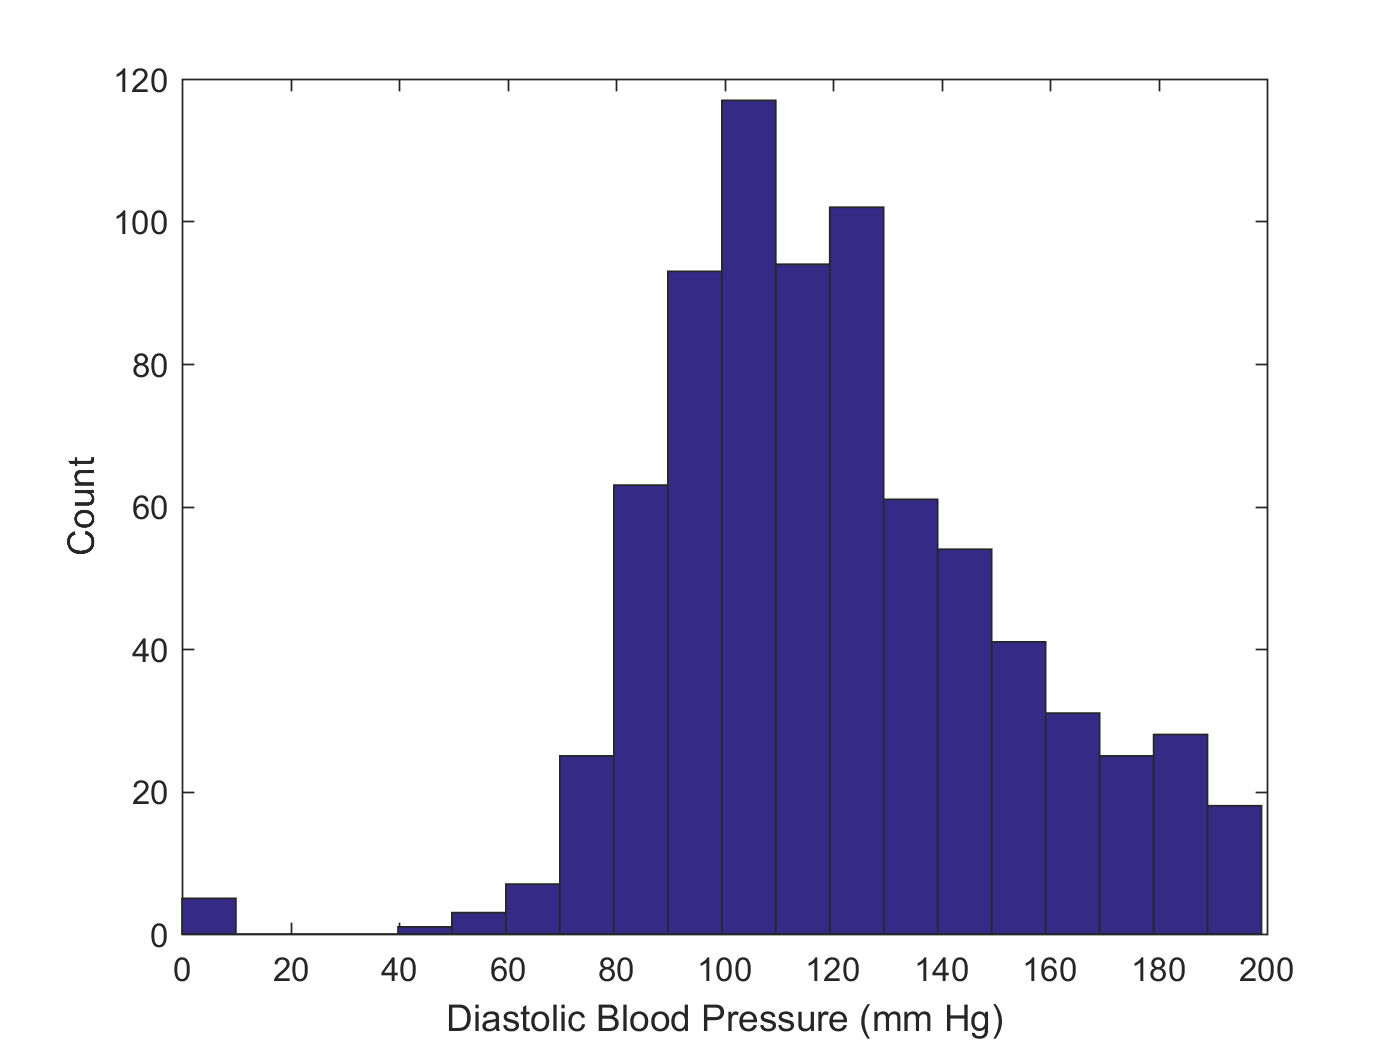
\includegraphics[width=18em]{p2e3.png} }}
	\qquad
	\subfloat[Figure 2]{{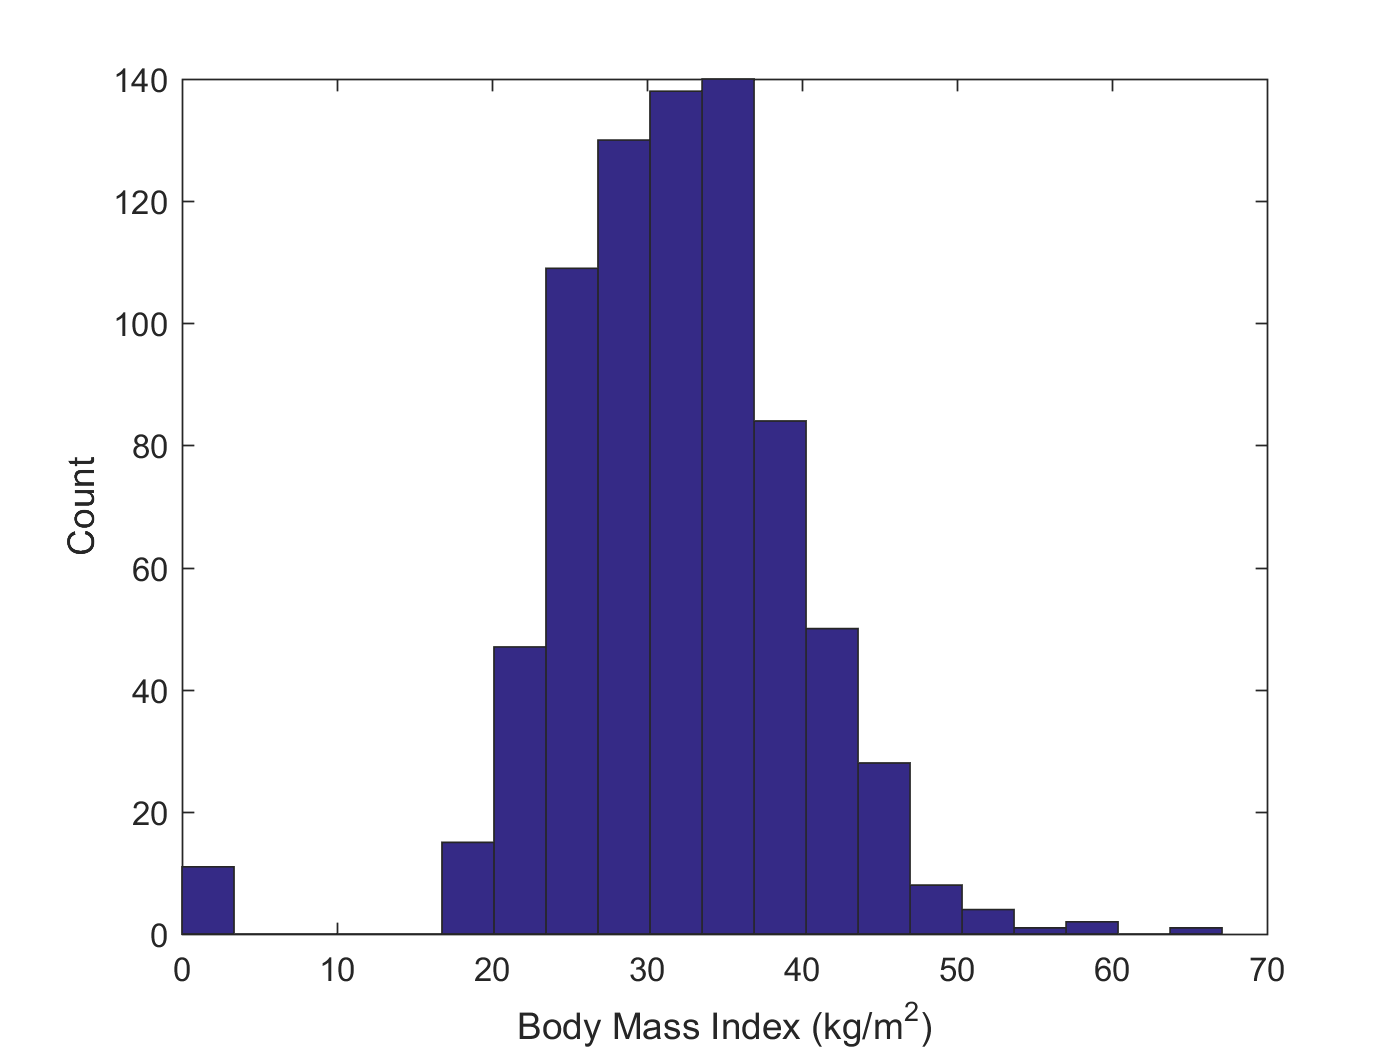
\includegraphics[width=18em]{p2e6.png} }}
	\label{fig:example}
\end{figure}

% F
\subsection{Subset Analysis}

Attribute 2 of the dataset, plasma glucose concentration after 2 hours in an oral glucose tolerance test, appears to be the most helpful in discriminating between the two sets. Based on the two histograms below, figure 4 represents a normal distribution for the negative diabetes test. However, as seen in figure 3, the distribution is heavily skewed to the right, indicating a correlation between glucose levels and positive test patients.

\begin{figure}[H]
	\captionsetup[subfigure]{labelformat=empty}
	\centering
	\subfloat[Figure 3]{{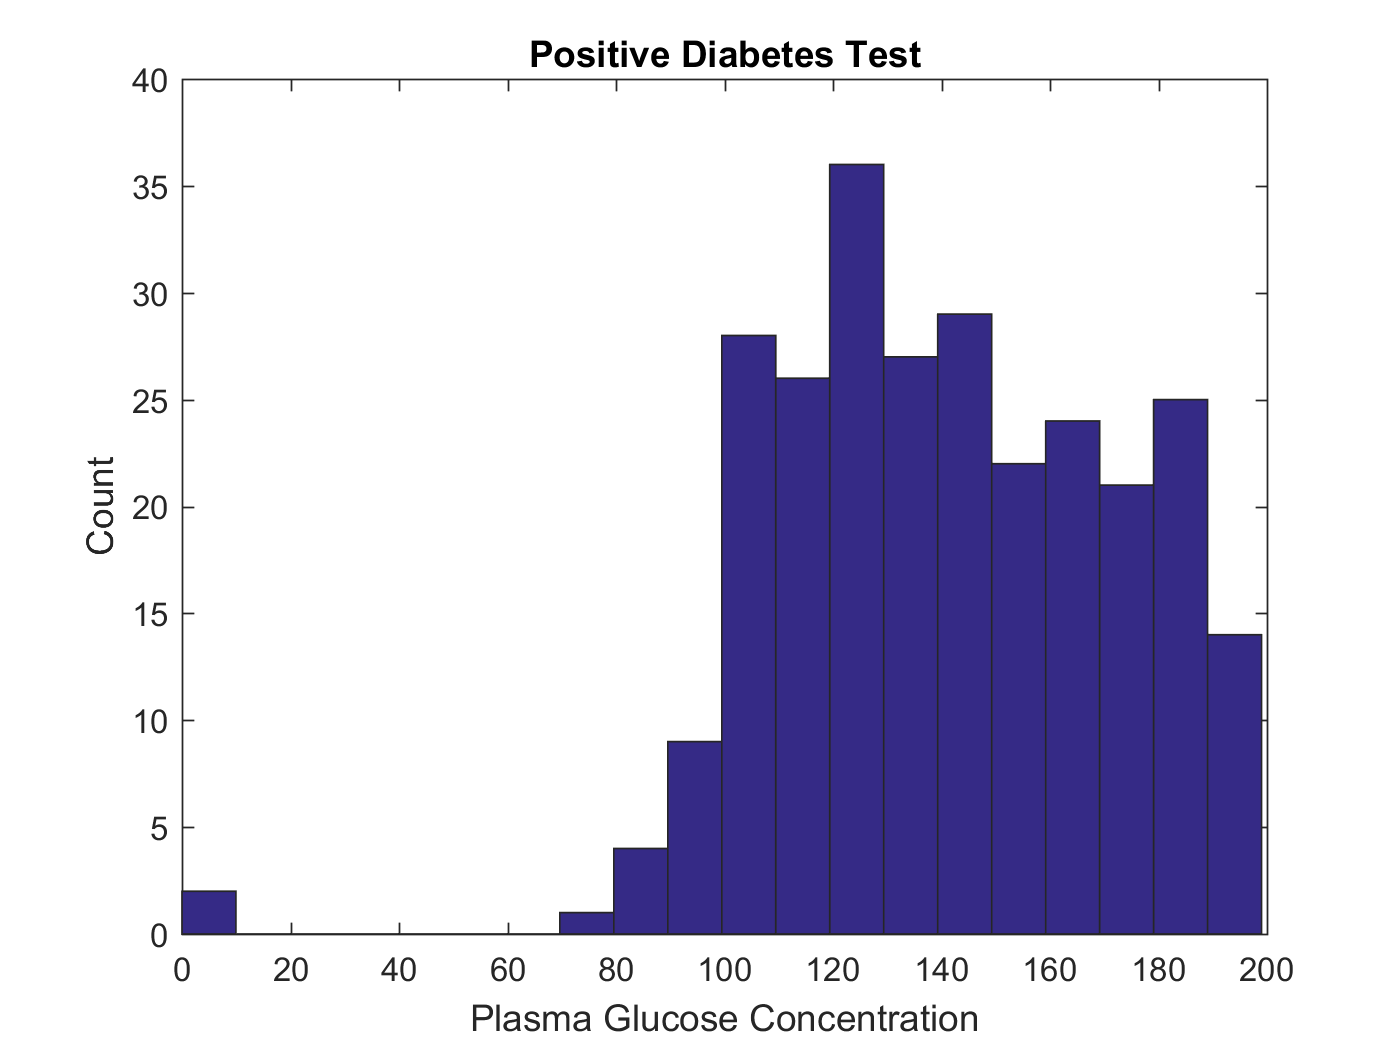
\includegraphics[width=18em]{p2f2d1.png} }}
	\qquad
	\subfloat[Figure 4]{{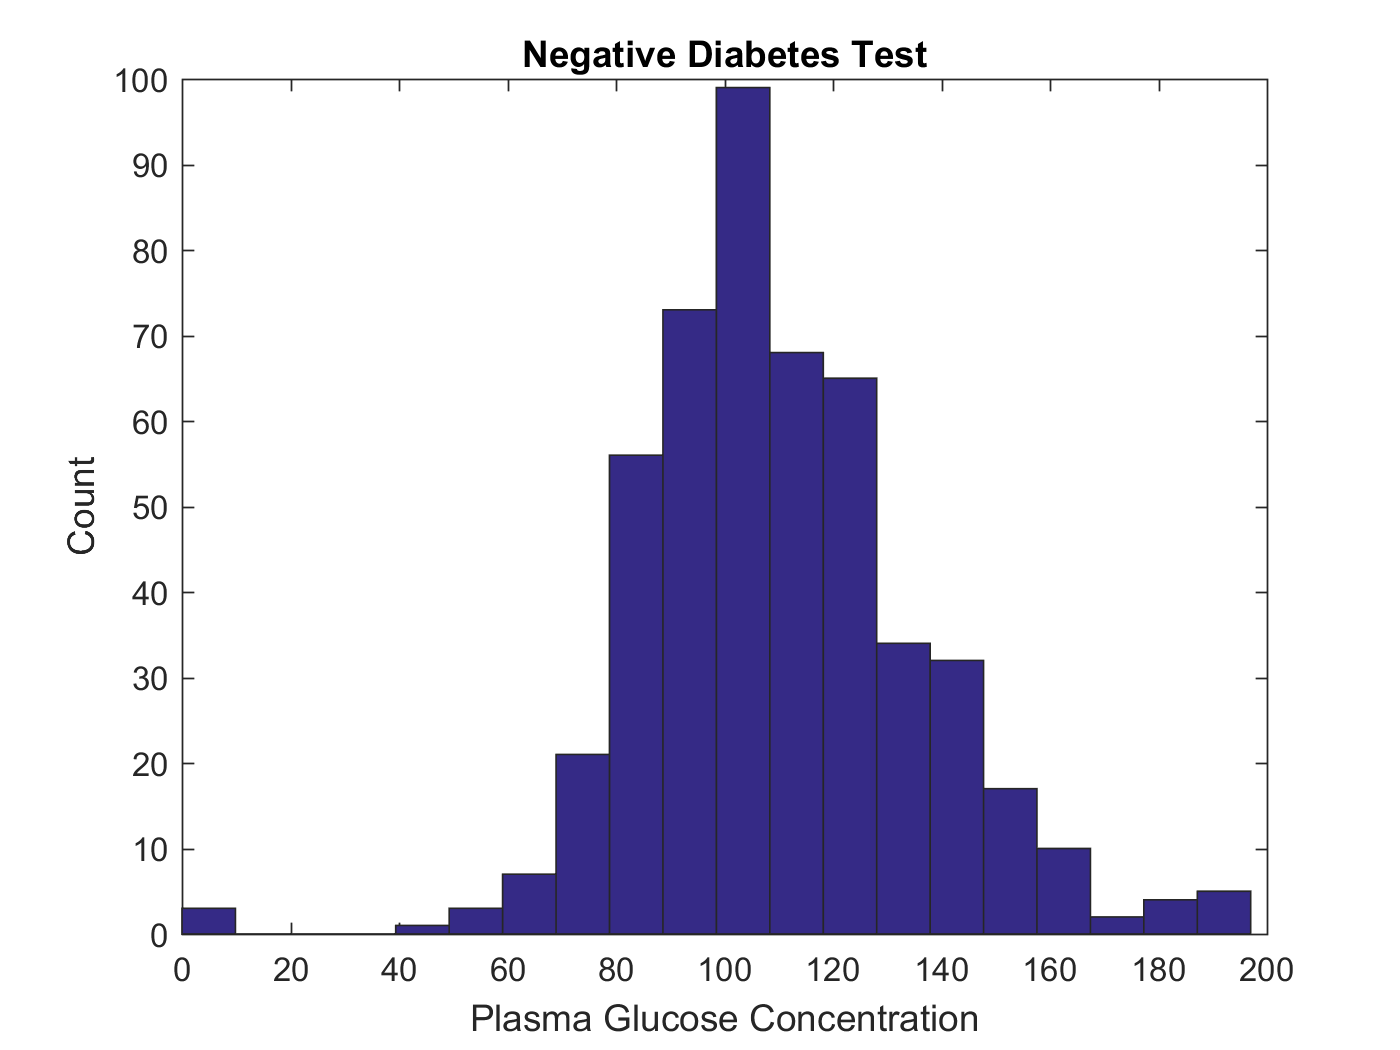
\includegraphics[width=18em]{p2f2d0.png} }}
	\label{fig:example}
\end{figure}

% G
\subsection{Scatter Plots}

\begin{verbatim}
function scatter_plot( vector )
    scatter( vector(:,1), vector(:,2) );
end
\end{verbatim}

Given two random variables that are independent, I would predict to see no correlation between the plotted values, which can be seen in figure 6. However, when these random variables are not quite independent, a correlation among the data points can be observed, as in figure 5. This is quite predictable in this example, as it is expected that those with a higher BMI would also tend toward a higher skin fold thickness due to the overlapping nature of the variables.

\begin{figure}[H]
	\captionsetup[subfigure]{labelformat=empty}
	\centering
	\subfloat[Figure 5]{{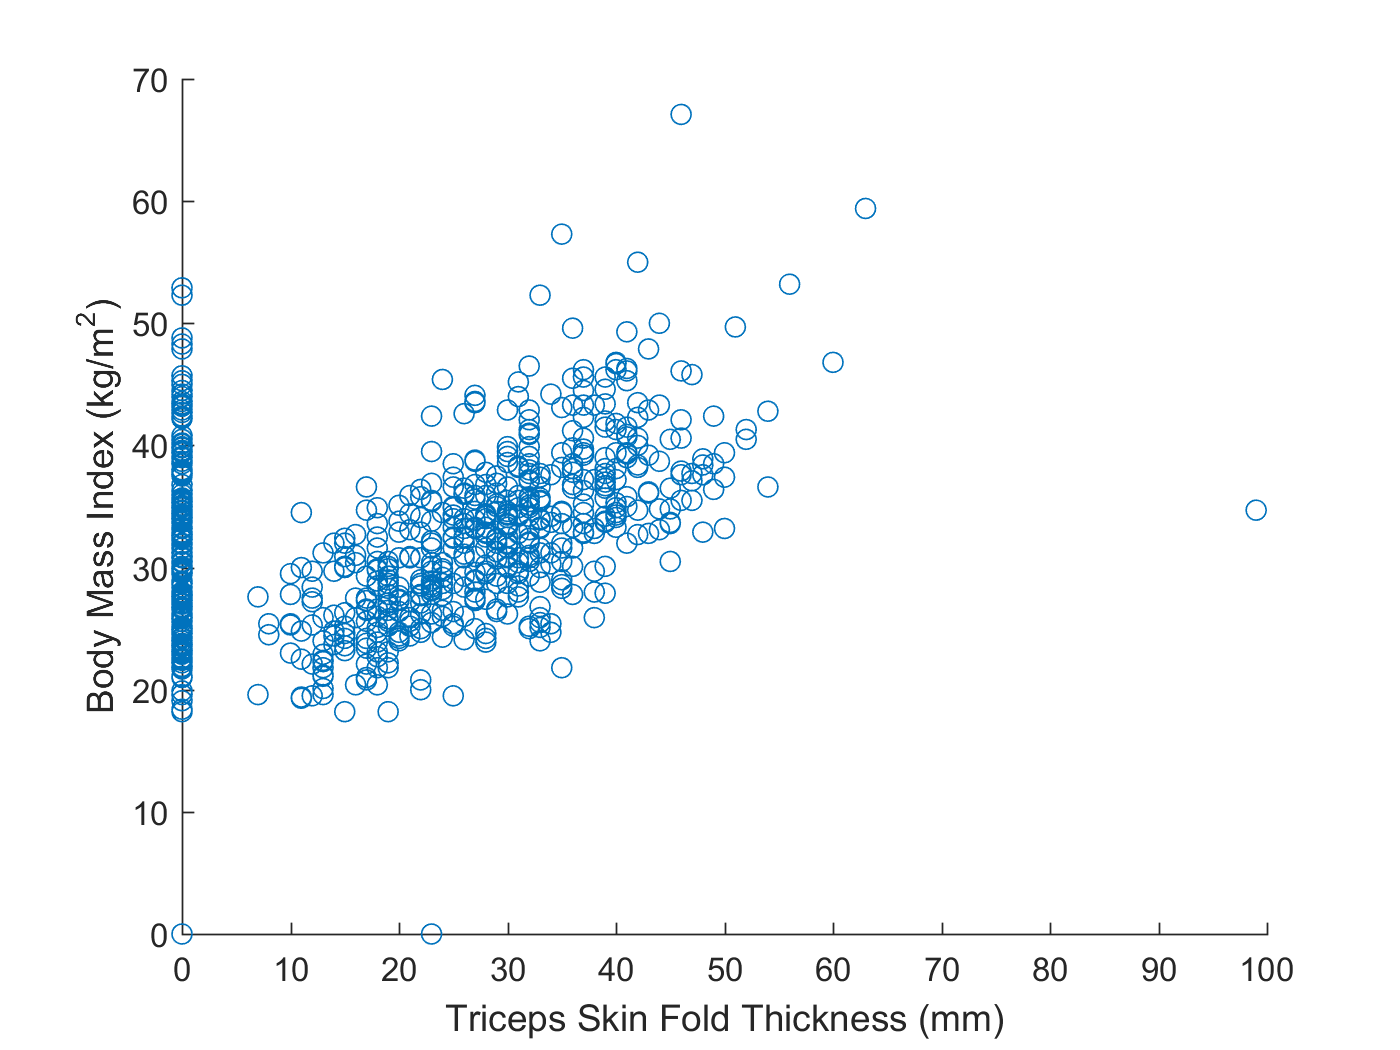
\includegraphics[width=18em]{p2g4v6.png} }}
	\qquad
	\subfloat[Figure 6]{{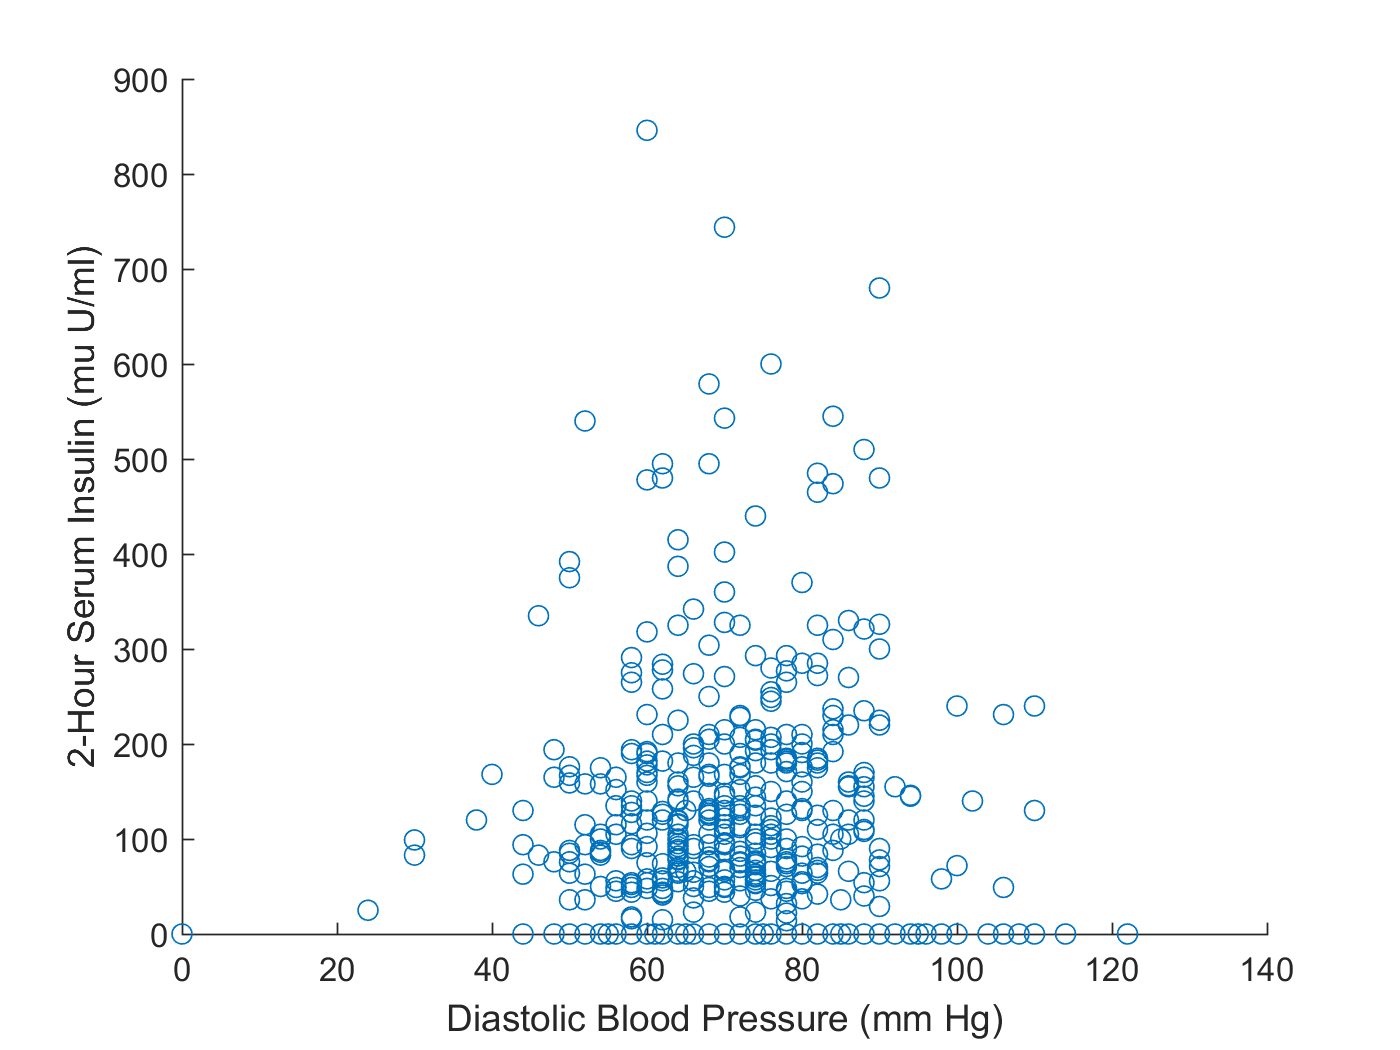
\includegraphics[width=18em]{p2g3v5.png} }}
	\label{fig:example}
\end{figure}

\section{Problem 3 - Data Preprocessing}

% A
\subsection{One's Hot Encoding}

One's hot encoding is a common scheme for encoding information utilizing standard binary values in a vector whereby the index of the '1' indicates the value of the scalar. Each subsequent scalar can be converted into its corresponding one's hot vector given the following encoding:
\begin{verbatim}
{brown, blue, white, red, yellow, orange, green, black}
\end{verbatim}

\begin{center}
	\begin{tabular}{ |l|l| } 
		\hline
		red & [0, 0, 0, 1, 0, 0, 0, 0] \\
		\hline
		black & [0, 0, 0, 0, 0, 0, 0, 1] \\
		\hline
		yellow & [0, 0, 0, 0, 1, 0, 0, 0] \\
		\hline
		red & [0, 0, 0, 1, 0, 0, 0, 0] \\
		\hline
		green & [0, 0, 0, 0, 0, 0, 1, 0] \\
		\hline
		blue & [0, 1, 0, 0, 0, 0, 0, 0] \\
		\hline
		blue & [0, 1, 0, 0, 0, 0, 0, 0] \\
		\hline
	\end{tabular}
\end{center}

% B
\subsection{Normalization}

\begin{verbatim}
function [ normalized, mu, sigma ] = normalize( attribute )
    mu = mean(attribute);    
    sigma = std(attribute);
    normalized = (attribute - mu)/sigma;
end
\end{verbatim}

First five values of Attribute 3 (Diastolic Blood Pressure) after being normalized.

\begin{center}
	\begin{tabular}{ |l|l|l|l|l|l| } 
		\hline
		0.1495 & -0.1604 & -0.2638 & -0.1604 & -1.5037 \\
		\hline
	\end{tabular}
\end{center}

% C
\subsection{Discretization}

\begin{verbatim}
function [ discrete ] = discretize_attribute( attribute, k )
    min_val = min(attribute);
    max_val = max(attribute);
    bin_div = (max_val - min_val)/k;
    discrete = fix((attribute-min_val)/bin_div);
end
\end{verbatim}

First five values of Attribute 3 (Diastolic Blood Pressure) after being discretized.

\begin{center}
	\begin{tabular}{ |l|l|l|l|l|l| } 
		\hline
		5 & 5 & 5 & 5 & 3 \\
		\hline
	\end{tabular}
\end{center}

\section{Problem 4 - Data Training}

\begin{verbatim}
function [ training_set, testing_set ] = divideset( dataset, p_train )

    training_count = round(p_train * length(dataset));
    indices = randperm(length(dataset), training_count);
    t = zeros([length(dataset) 1]);
    t(indices) = 1;

    training_set = dataset(t(:) == 1,:);
    testing_set = dataset(t(:) == 0,:);

end
\end{verbatim}

\section{Problem 5 - Matrix Operations}

\subsection{$A^{T}$}
\begin{center}
	\begin{tabular}{ |l|l| } 
		\hline
		1 & 3 \\
		\hline
		2 & 4 \\
		\hline
		5 & 6 \\
		\hline
	\end{tabular}
\end{center}

\subsection{$B^{-1}$}
\begin{center}
	\begin{tabular}{ |l|l|l| } 
		\hline
		1 & -5.5 & 1.25 \\
		\hline
		0 & -0.5 & 0.25 \\
		\hline
		-0.667 & 4.333 & -1 \\
		\hline
	\end{tabular}
\end{center}

\subsection{$B + C$}
\begin{center}
	\begin{tabular}{ |l|l|l| } 
		\hline
		15 & 7 & 14 \\
		\hline
		3 & -1 & 7 \\
		\hline
		3 & 6 & 10 \\
		\hline
	\end{tabular}
\end{center}

\subsection{$B - C$}
\begin{center}
	\begin{tabular}{ |l|l|l| } 
		\hline
		-1 & -5 & 4 \\
		\hline
		1 & 5 & -1 \\
		\hline
		5 & 10 & 2 \\
		\hline
	\end{tabular}
\end{center}

\subsection{$A * B$}
\begin{center}
	\begin{tabular}{ |l|l|l| } 
		\hline
		31 & 45 & 45 \\
		\hline
		53 & 59 & 75 \\
		\hline
	\end{tabular}
\end{center}

\subsection{$B * C$}
\begin{center}
	\begin{tabular}{ |l|l|l| } 
		\hline
		48 & 21 & 75 \\
		\hline
		15 & 0 & 30 \\
		\hline
		34 & -12 & 76 \\
		\hline
	\end{tabular}
\end{center}

\subsection{$B * A$}
Cannot compute matrix operation because inner dimensions do no match.

\end{document}          
